\section{Desarrollo del proyecto}
En esta sección repasaremos los aspectos principales y las especificaciones seguidas 
en el desarrollo de este proyecto. Los principales subtemas que se abordarán son la 
especificación y requisitos del proyecto, el enfoque que se tomó hacia la arquitectura 
y el diseño, una breve inmersión en las tecnologías que se utilizaron, la estrategia de 
pruebas seguida durante el proyecto, consideraciones sobre el entorno de trabajo donde 
se realizó el desarrollo y por último si hubo algún incidente durante el desarrollo.

\subsection{Especificación de Requisitos del Sistema}

\subsubsection{Stakeholders}
Dado que este proyecto es de indole de academica sobre como aplicar 
tecnicas de IL en problemas NP-Hard no tiene clientes directos. Sin embargo, 
teniendo en cuenta hacia qué está enfocado y la utilidad del mismo, se pueden 
identificar 2 tipos de grupos de interes. En primer lugar, los investigadores 
dentro de Tecnalia, ya que un avance en esta problematica les puede servir como punto de partida
para mejorar sus propios algoritmos. En segundo lugar, los clientes de Tecnalia,
ya que podrán utilizar esta herramienta para resolver sus propios problemas de
optimización con unos pequeños ajustes.

\subsubsection{Restricciones Obligatorias}
\begin{itemize}
    \item \textbf{Limitación de tecnologías:} el proyecto esta limitado al uso de
    tecnologías y/o herramientas de código abierto o con licencias apropiadas.
    \item \textbf{Limitación de recursos:} el proyecto esta limitado 
    por recursos como el tiempo, el presupuesto, la disponibilidad de personal, 
    el equipo de hardware y software.
    \item \textbf{Requisitos legales y éticos:} el proyecto esta limitado 
    por los requisitos legales y éticos que deben cumplirse, por ejemplo, en lo 
    que respecta a la privacidad de los datos, la seguridad, la propiedad intelectual 
    y la ética en la investigación.
    \item \textbf{Limitación de acceso a datos:} el proyecto esta limitado
    por el acceso a los datos de los clientes de Tecnalia. En este caso, se
    utilizarán datos generados sinteticamente para poder realizar el proyecto.
\end{itemize}

\subsubsection{Reglas de Negocio}
\begin{itemize}
    \item Al aplicar la metodologia se deben incluir reglas 
    de validación para garantizar que los datos de entrada sean coherentes 
    y estén dentro de los límites aceptables para el problema a resolver.
    \item Se deben establecer los parámetros y procedimientos para el proceso 
    de entrenamiento del modelo de aprendizaje automático que se utilizará 
    para la resolución del problema, incluyendo los criterios de evaluación del modelo.
    \item Se deben especificar las reglas para la interpretación de los resultados 
    obtenidos por la metodología, así como las medidas de calidad que se utilizarán 
    para evaluar el rendimiento de la solución propuesta.
    \item La metodología debe incluir reglas para la gestión de errores
    de la metodología, incluyendo la revisión periódica de las reglas de negocio 
    y la actualización de los modelos de aprendizaje automático.
\end{itemize}
\subsubsection{Catálogo de Requisitos Funcionales}
\begin{enumerate}
    \renewcommand{\labelenumi}{RF\arabic{enumi}}
    \item Se debe proporcionar una definicion clara de los objetivos de la investigación 
    y cómo se van a alcanzar.
    \item Aplicando la metodología debe ser capaz de generar el conjunto de datos de entrenamiento
    y validacion a partir de sistemas de generación de instancias aleatorias.
    \item La metodología debe idenficar diferentes formas para encontrar un experto
    que pueda generar soliciones optimas del caso de uso del problema.
    \item La metodología debe incluir el diseño y entrenamiento de un modelo de Machine Learning 
    adecuado para la tarea específica, de manera que se optimice su precisión y eficiencia.
    \item Aplicando la metodología debe ser capaz de medir y evaluar el rendimiento del modelo 
    utilizando una o varias metricas de calidad específicas para el caso en concreto.
    \item La metodología debe proporcionar un marco para el diseño de la investigación, 
    incluyendo la definición de variables, la identificación de las fuentes de datos y 
    la elección de los métodos de recolección de datos.
    \item La metodología debe incluir la interpretación de los resultados del modelo 
    de Machine Learning, de manera que se puedan extraer conclusiones útiles y relevantes.
\end{enumerate}

\subsubsection{Requisitos no Funcionales}
\begin{enumerate}
    \renewcommand{\labelenumi}{RNF\arabic{enumi}}
    \item La metodología debe ser fácil de entender y utilizar tanto para 
    investigadores expertos como para aquellos que no tienen experiencia en el campo.
    \item La metodología debe ser reproducible por otros investigadores, de manera 
    que los resultados obtenidos puedan ser comparados y validados.
    \item La metodología debe ser lo suficientemente flexible para adaptarse a 
    diferentes situaciones y contextos de investigación.
    \item La metodología debe ser clara y precisa en su presentación y explicación, 
    para evitar ambigüedades y malinterpretaciones.
    \item La metodología debe ser innovadora y estar actualizada con los últimos 
    avances en investigación y tecnología. 
    \item Al desrrolar la metodología se deben seguir los principios de código limpio, 
    utiliar una arquitectura adecuadas y patrones de diseños cuando sea necesario.
\end{enumerate}
\subsection{Especificación del Diseño}
\subsubsection{Arquitectura y entorno tecologico del proyecto}
\paragraph{Arquitectura del software}
La arquitectura del software del modelo está compuesta por cuatro capas principales: 
la capa del modelo, la capa del estado compuesto por un grafo, la capa del 
environment y la capa de ejecución. Se puede ver un diagrama de la arquitectura en la
figura \ref{fig:layers}. \medskip

\begin{itemize}
    \item \textbf{Capa de ejecución:} Esta capa se encarga de ejecutar todo el ecosistema
    del modelo. En nuestro caso es ejecutada por Python 3.10.6 y ofrece la versatilidad de
    poder ejecutar el modelo ya sea en un entorno local o en la nube. 
    \item \textbf{Capa del environment:} Esta capa se encarga de generar el entorno en el que se
    ejecutará el modelo. Cuando se va a resolver un problema de scheduling, el entorno
    prepara todo lo necesario para que el modelo pueda interactuar con el problema y le
    proporciona toda la información necesaria para que pueda tomar decisiones.
    \item \textbf{Capa del estado:} Esta capa se encarga de representar el estado del problema
    mediante un grafo. El grafo representa todas las operaciones que se deben ejecutar y
    las restricciones que existen entre ellas.
    \item \textbf{Capa del modelo:} Esta capa se encarga de resolver el problema de scheduling
    mediante un modelo de Deep Learning. El modelo recibe como entrada el grafo del
    estado y genera como salida una asignación de las operaciones a los recursos. 
\end{itemize}

\begin{figure}[ht]
    \centering
    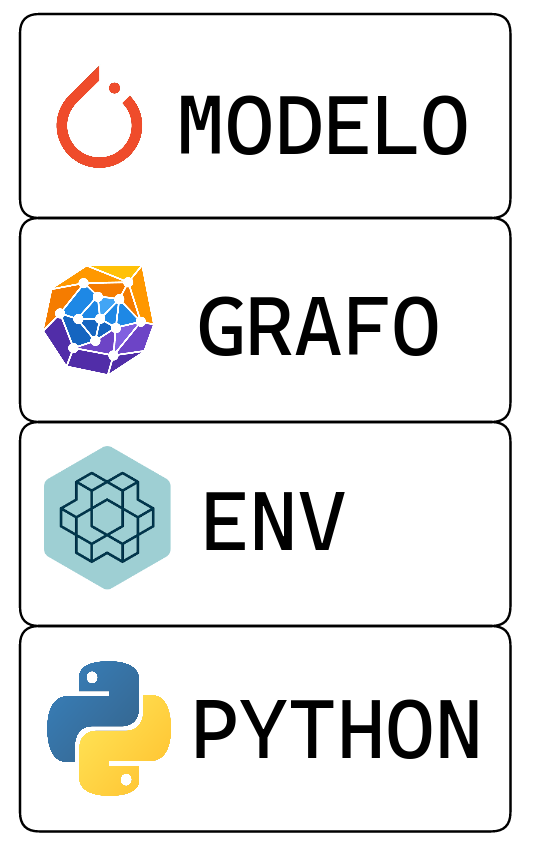
\includegraphics[scale=0.27]{layers.png}
    \caption{Capas de la arquitectura}
    \label{fig:layers}
\end{figure}


\paragraph{Despliegue fisico}
La visualización de los resultados es una parte crítica e importante del proceso. Permite 
a los usuarios finales entender y analizar los datos de una manera más efectiva.  
Sin embargo, es importante destacar que esta parte del proyecto es 
estrictamente opcional y dependerá de las necesidades concretas del caso de uso. 
Si bien la visualización del problema puede ser extremadamente útil algunos casos, puede que no sea 
relevante o necesaria en otros. Por lo tanto, se debe evaluar cuidadosamente la necesidad de 
esta visualización antes de implementarla, ya que puede ser un proceso costoso y 
requerir mucho tiempo.\medskip

\begin{figure}[ht]
    \centering
    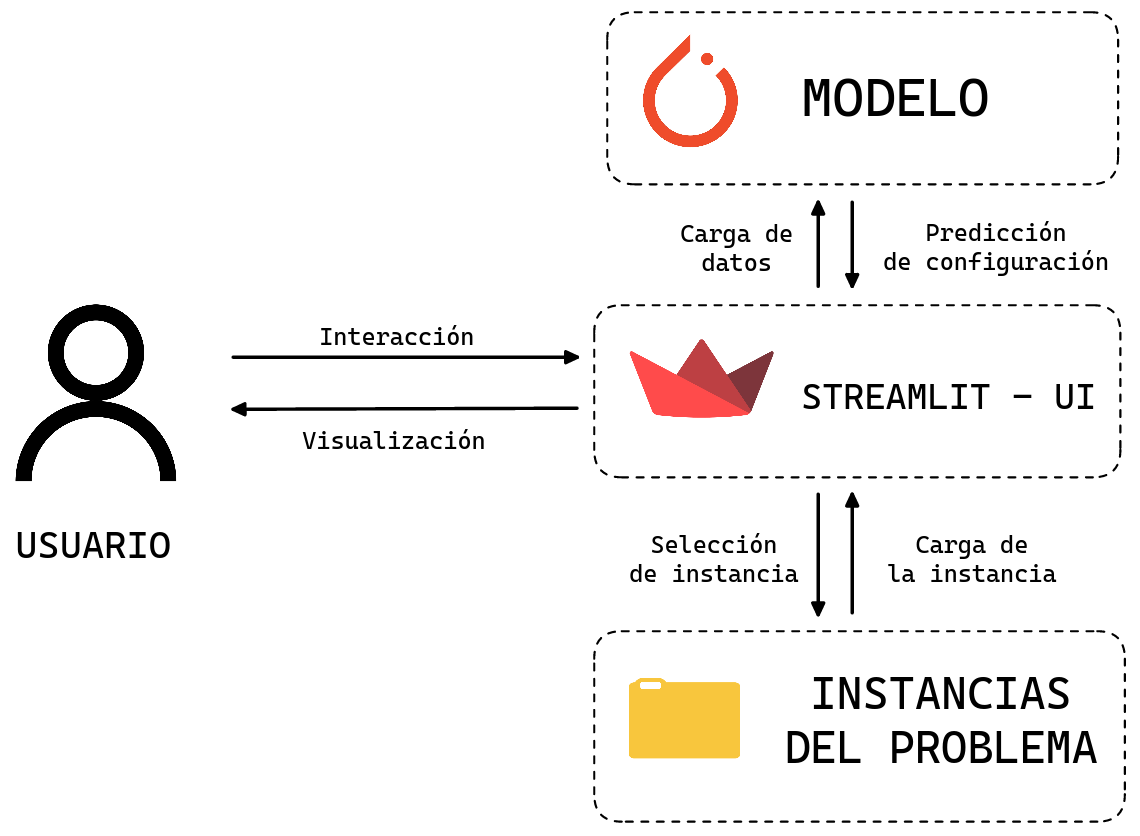
\includegraphics[scale=0.25]{deploy.png}
    \caption{Arquitectura fisica}
    \label{fig:despliegue}
\end{figure}

En este proyecto en particular, se ha optado por se crear una aplicacion web en Streamit 
desde la cual mediante una llamada al modelo generar un gráfico Gantt en el que se podra
visualizar todas las operaciones y sus respectivas asigncaciones y tiempos de ejecucion.
En la figura \ref{fig:despliegue} se puede ver un diagrama del despliegue fisico del modelo.
La aplicacion sirve como intermediario entre el usuario y el modelo, para ello extrae las
diferentes configuraciones de problemas desde una carpeta en la que se encuentran los 
archivos. Lo importante de esta distribucion es que permite una gran versatilidad a la hora
de ejecutar el modelo, ya que se podría mover la ejecución del modelo a un microservicio
externo que se encargue de ejecutar el modelo y devolver los resultados a la aplicacion web.
Para ver más información sobre la aplicación web, se puede consultar el apartado de manual
de usuario donde se explica con más detalle. 

\subsubsection{Descripcion del diseño}
Uno de los diseños más comunmente utilizados para resolver problemas de machine learning
es el uso de sistemas de pipelines. Estos sistemas escapan del paradigma tradicional de
programación secuencial y se basan en la idea de que el problema se puede resolver
mediante la composición de una serie de pasos o etapas. Cada etapa se encarga de realizar
una tarea específica y se comunica con las demás mediante un sistema de colas. De esta
manera, se puede lograr un sistema altamente escalable y flexible. Además, se puede
reutilizar cada etapa para diferentes pipelines o enlazar diferentes pipelines para
conseguir uno más complejo. Otra de las ventajas de este diseño es que permite
abstraer la implementación de cada etapa, lo que permite que cada una de ellas se pueda
mejorar o cambiar sin afectar al resto de ellas, siempre y cuando se mantenga la
interfaz de comunicación.

\subsubsection{Modelo de diseño}
\begin{figure}[ht]
    \centering
    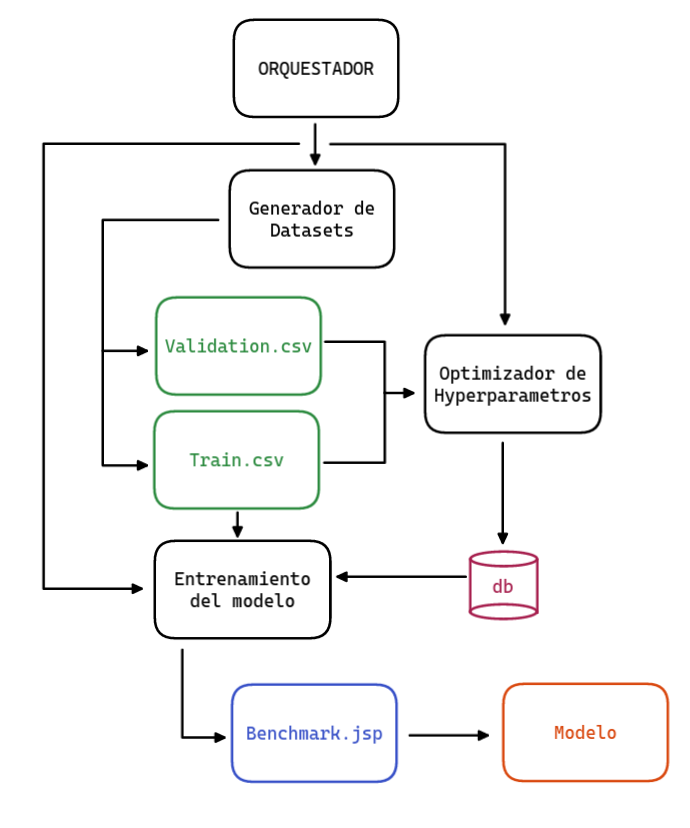
\includegraphics[scale=0.35]{disenio.png}
    \caption{Diseño del sistema}
    \label{fig:desing}
\end{figure}

En la figura \ref{fig:desing} se puede ver al completo las diferentes etapas que componen
el sistema. 

\subsection{Tecnologías Utilizadas}
En la sección se presentarán todas las tecnologías que han tenido un impacto directo en el desarrollo de las 
funcionalidades del proyecto de Machine Learning.

\subsubsection{Python}
Python \cite{C8d} es un lenguaje de programación interpretado de alto nivel. Es una de las herramientas más populares 
en la comunidad de Data Science y Machine Learning debido a su facilidad de uso, su amplia gama de bibliotecas 
y su enfoque en la legibilidad del código. Además, recientemente se está haciendo una tarea de mejora del 
lenguaje con la inclusión de nuevas librerías basadas en C para un mejor rendimiento, inclusión de elementos 
de tipado estático para el mantenimiento del código y mejoras en el sistema de errores.

\subsubsection{NumPy}
NumPy \cite{Numpy} es una biblioteca de Python utilizada para trabajar con matrices y arrays multidimensionales de manera 
eficiente. Fue desarrollada en C++ para ser utilizada en aplicaciones de Data Science y matemáticas, ofrece 
una amplia variedad de funciones y herramientas para operar con matrices y realizar cálculos numéricos complejos. 
Además, al estar escrito en C++ está altamente optimizado para trabajar con grandes conjuntos de datos, realizar 
operaciones aritméticas y lógicas, de indexar y redimensionar matrices de manera eficiente, realizar transformaciones 
de Fourier y realizar cálculos de álgebra lineal.

\subsubsection{Pandas}
Pandas \cite{pandas} es una biblioteca de Python utilizada para la manipulación y análisis de datos. Es especialmente 
útil para el manejo de grandes conjuntos de datos y ofrece una variedad de herramientas y funciones para 
trabajar con diferentes tipos de datos y formatos. Una de las estructuras de datos principales de Pandas es 
el DataFrame, que se puede considerar como una tabla de datos bidimensional, donde cada fila representa una 
observación y cada columna representa una variable. Los DataFrames permiten la manipulación y transformación 
de datos mediante una variedad de operaciones, lo que los hace muy útiles en aplicaciones de ciencia de datos 
y análisis de datos. 

\subsubsection{PyTorch}
PyTorch \cite{PyTorch} es un framework de código abierto de Deep Learning hecho en Python, desarrollado por el equipo 
de Inteligencia Artificial de Facebook. Se utiliza para crear y entrenar modelos de redes neuronales para resolver 
problemas de Machine learning. PyTorch es muy popular en la comunidad de investigación debido a su facilidad de uso 
y su capacidad para realizar cálculos en GPU para acelerar el proceso de entrenamiento de modelos. Además, PyTorch
ofrece una gran variedad de herramientas y funciones para trabajar con redes neuronales, como la creación de
diferentes tipos de redes neuronales, la definición de funciones de pérdida, la definición de optimizadores, la 
definición de funciones de activación, etc.

\subsubsection{Gym}
Gym \cite{Gym} es una biblioteca de Python utilizada para el diseño y creación de environments de RL. Incluye un 
gran conjunto de herramientas para trabajar con algoritmos personalizados y ofrece muchas facilidades en 
el registro y monitorización del proceso de entrenamiento. Todas estas razones lo convierte en la opción más popular 
para los desarrolladores cuando abordan problemas de RL.

\subsubsection{PyTorch Geometric}
PyTorch Geometric \cite{pytorch-geometric} es una librería que ofrece soporte para el procesamiento de grafos, lo que significa 
que se puede utilizar para trabajar con redes de datos en las que los nodos están conectados por enlaces. 
Esto puede ser útil ya que mediante técnicas de Deep Learning se puede analiza la estructura y las 
relaciones que existen entre los nodos de un grafo y extraer de ahi sus características. Además, la 
librería ofrece herramientas para trabajar con diferentes tipos de grafos, como grafos dirigidos y heterogéneos, 
que son los utilizados en el proyecto, y proporciona una serie de funciones para realizar 
operaciones básicas con grafos.

\subsubsection{Or-tools}
OR-Tools \cite{ortools} es una biblioteca de optimización combinatoria de código abierto para Python y otros 
lenguajes de programación. Permite resolver problemas de optimización de manera eficiente, utilizando una 
amplia variedad de algoritmos y técnicas de programación matemática. Con OR-Tools, los usuarios pueden 
resolver problemas de programación lineal, programación entera mixta, programación cuadrática, 
problemas de rutas y muchos otros. Además, la biblioteca también incluye herramientas para resolver 
problemas de programación con restricciones, como la asignación de tareas o la programación de horarios.

\subsubsection{Optuna}
Optuna \cite{optuna_2019} es una biblioteca de optimización de hiperparámetros de código abierto para Python. Su objetivo 
es automatizar el proceso de ajuste de hiperparámetros, que a menudo es un proceso intensivo en 
recursos y muy demandante en tiempo, para permitir a los usuarios encontrar la mejor configuración 
de hiperparámetros de sus modelos de Machine Learning de manera eficiente. Optuna utiliza algoritmos 
de optimización Bayesiana \cite{Ye_2020} para buscar los mejores valores de hiperparámetros en función del 
rendimiento de los modelos en el conjunto de validación. Con Optuna, los usuarios pueden definir una función 
objetivo y especificar los rangos de búsqueda de cada hiperparámetro, así como las restricciones entre ellos, 
lo que permite a la biblioteca ajustar varios hiperparámetros al mismo tiempo.

\subsubsection{Streamlit}
Streamlit \cite{Streamlit} es una biblioteca de Python que permite a los usuarios crear aplicaciones web interactivas
para Machine Learning y Data Science. Proporciona una serie de herramientas y widgets preconstruidos 
que permiten a los desarrolladores agregar fácilmente gráficos, tablas, mapas y otros tipos de 
visualizaciones a sus aplicaciones. Además, se integra bien con bibliotecas populares de Python 
para el procesamiento de datos y el aprendizaje automático, como Pandas, NumPy y Scikit-Learn \cite{scikit-learn}.
Streamlit se ejecuta en un servidor local y los usuarios interactúan con la aplicación a través 
de un navegador web. Esto hace que sea fácil compartir aplicaciones y colaborar en ellas.
\subsection{Consideraciones sobre la Implementación}
\subsubsection{Estructura del codigo}
La estructura del codigo se ha diseñado para que sea lo más modular posible,
de forma que cada modulo tenga una única responsabilidad y sea fácilmente
intercambiable. La distribucion de ficheros y carpetas se puede ver en la 
\textbf{Figura \ref{fig:estrcutra-ficheros}}.

\begin{figure}[ht]
\dirtree{%
    .1 /.
    .2 Makefile.
    .2 README.md.
    .2 pyproject.toml.
    .2 .pre-commit-config.yaml.
    .2 requirements.txt.
    .2 src.
    .3 \_\_init\_\_.py.
    .3 app.py.
    .3 main.py.
    .3 config.
    .4 hyperparams.py.
    .4 settings.py.
    .3 environment.
    .4 fjspenv.py.
    .4 generator.py.
    .4 graph.py.
    .4 solver.py.
    .3 model.
    .4 actor.py.
    .4 eval\_model.py.
    .4 train\_model.py.
    .3 pipes.
    .4 generate\_data.py.
    .4 generate\_optimun.py.
    .4 generate\_training.py.
    .4 generate\_validation.py.
    .3 utils.
    .4 parsedata.py.
    .2 test.
    .3 fjspenv\_test.py.
    .3 graph\_test.py.
    .3 pipeline\_test.py.
}
\caption{Estructura de ficheros del proyecto}
\label{fig:estrcutra-ficheros}
\end{figure}

A continuación se detallan las carpetas y ficheros más importantes del proyecto:
\begin{itemize}
    \item \textbf{src: } Contiene todo el código ejecutable del proyecto, siendo \textit{main.py} el archivo 
    principal que se ejecuta para lanzar el proyecto. Este archivo se encarga de cargar los
    diferentes módulos y realizar las llamadas a las pipelines para generar los datos de entrenamiento,
    validación, así como ejecutar el entrenamiento y la evaluación del modelo. También existe un archivo
    \textit{app.py} que se encarga de cargar la demo del proyecto mediante una pagina web y ejecutar el 
    algoritmo de resolución.
    \item \textbf{config: } Contiene el archivo de configuración de los hiperparámetros para el entrenamiento 
    y las diferentes variables de configuración del proyecto.
    \item \textbf{environment: } Contiene los archivos relacionados con el environment del problema, como la
    clase que representa el grafo heterogeneo, el environment de OpenAI Gym, el generador de instancias y 
    el resolutor de las mismas.
    \item \textbf{model: } Contiene los archivos relacionados con el modelo de aprendizaje profundo, como la
    clase que representa la red neuronal, el entrenador y el evaluador del modelo.
    \item \textbf{pipes: } Contiene los archivos relacionados con las pipelines de generación de datos,
    validación y entrenamiento. 
    \item \textbf{utils: } Contiene los archivos de utilidades, como el parser de los datos de entrada.
    \item \textbf{test: } Contiene los archivos de testeo de los módulos.
\end{itemize}

\subsubsection{Entorno de desarrollo}
El desarrollo del proyecto se ha realizado en un entorno Linux, concretamente en un sistema operativo
Arch Linux. El editor de código utilizado ha sido Visual Studio Code, que es un editor de código
de código abierto desarrollado por Microsoft. Este editor de código es uno de los más utilizados
en la actualidad y cuenta con una gran comunidad de desarrolladores que desarrollan extensiones
para el mismo. En este proyecto se ha utilizado la extensión de Python para Visual Studio Code,
que permite ejecutar código Python directamente desde el editor de código, así como depurar el
código y ejecutar tests. También se ha utilizado otras extensiones como GitHub Copilot, que es
una extensión que utiliza inteligencia artificial para sugerir código al desarrollador y amVim
que es una extensión que permite utilizar el editor de código como si fuera el editor Vim.

\subsubsection{Gestión de dependencias y reproducibilidad}
La gestión de dependencias y la reproducibilidad es uno de los temas de mayor importancia en el 
desarrollo de un proyecto de software. En el caso de este proyecto, se ha optado por utilizar 
un kit de herramientas para garantizar que el proyecto se pueda ejecutar siempre en las mismas 
condiciones. Para ello, se va ha fijar la versión de Python a la 3.10.6 y el resto de dependencias. 

\begin{itemize}
    \item \textbf{Pyenv: } Pyenv es un administrador 
    de versiones de Python que permite tener múltiples versiones de Python instaladas en un mismo sistema 
    y cambiar fácilmente entre ellas. Con Pyenv, es posible instalar distintas versiones de 
    Python y asegurarse de que el código se está ejecutando en la versión correcta. 
    
    \item \textbf{Virtualenv: } Virtualenv es una herramienta que permite crear entornos virtuales de Python para trabajar 
    en proyectos específicos. Cada entorno virtual puede tener su propia versión de Python y bibliotecas instaladas, 
    lo que permite aislar proyectos y evitar conflictos entre versiones y dependencias. Con Virtualenv, 
    es posible instalar y gestionar paquetes de Python específicos para cada proyecto, sin afectar 
    al sistema operativo global.

    \item \textbf{Pip-Tools: } Pip-Tools es una herramienta de línea de comandos para la gestión de 
    dependencias de Python. Permite especificar las dependencias de un proyecto en un archivo 
    "pyproject.toml" y asegurarse de que se instalen y se mantengan actualizadas todas las dependencias 
    de manera controlada. También permite generar archivos "requirements.txt" en el que se especifican las 
    versiones exactas de todas las dependencias, lo que ayuda a garantizar que la reproducibilidad del 
    proyecto se mantenga consistentes y se instalen correctamente.

\end{itemize}


\subsubsection{Gestión de la calidad del codigo}
Al igual que la gestión de dependencias, la gestión de la calidad del código es un tema de gran importancia
ya que permite mantener un código limpio, legible y fácil de mantener. Para ello, se ha optado por utilizar
una serie de medidas y herramientas que permiten mantener la calidad del código a lo largo del desarrollo del proyecto.
Entre estas medidas se incluyen liteners de código, formateadores de código, analizadores estáticos de código y
herramientas de pruebas unitarias. A continuación se detallan la lista de herramientas:

\begin{itemize}
    \item \textbf{Git: } Git es un sistema de control de versiones distribuido que se utiliza para el 
    seguimiento y gestión del código fuente. Permite a los desarrolladores trabajar en el mismo código fuente 
    sin necesidad de coordinar su trabajo constantemente. Ofrece la posibilidad de volver a versiones anteriores en 
    caso de errores o cambios no deseados, paralelismo de trabajo mediante el uso de diferentes ramas y cuenta 
    con multitud de plataformas web como Github o Gitlab para el almacenamiento de repositorios en remoto.

    \item \textbf{Pre-commit: } Pre-Commit es una herramienta que se utiliza para garantizar que el código 
    fuente de un proyecto cumpla con un conjunto de reglas y estándares de calidad antes de que se realice 
    un commit. Pre-Commit se integra con Git y se ejecuta automáticamente antes de cada commit, lo que ayuda 
    a garantizar que el código se mantenga limpio y organizado. Se configura mediante un archivo llamado 
    ".pre-commit-config.yaml", que especifica las herramientas que se utilizarán para verificar el código 
    y viene con una gran cantidad de herramientas integradas, incluyendo linters de Python, comprobadores 
    de estilo de código, herramientas de seguridad, etc. También es posible agregar herramientas 
    personalizadas si es necesario.

    \item \textbf{Ruff:} Ruff es un linter de Python escrito en Rust, es decir una herramienta de 
    análisis estático de código que ayuda a identificar errores de sintaxis, errores de estilo y posibles 
    problemas de rendimiento en el código fuente de un programa. Además, el hecho de que RUFF esté escrito 
    en Rust le da una ventaja en cuanto a velocidad y eficiencia, el uso de Rust significa que RUFF se 
    ejecutará rápidamente y consumirá pocos recursos del sistema, lo que puede ser especialmente beneficioso 
    para proyectos de gran tamaño.

    \item \textbf{Black: } Black es un formateador de código para Python que se utiliza para garantizar
    que el código cumpla con las directrices de estilo de Python PEP 8, lo que mejora la legibilidad 
    del código y ahorra tiempo de desarrollo. Se integra fácilmente en flujos de trabajo existentes 
    y es altamente configurable para adaptarse a diferentes estilos de formato. Black es compatible 
    con diferentes versiones de Python y es una herramienta valiosa para cualquier equipo de desarrollo 
    de Python que busque mejorar la calidad y consistencia del código.

    \item \textbf{Mypy: } Mypy es una herramienta de análisis estático para Python que permite a los 
    desarrolladores verificar el tipado estático de su código. Al analizar el código para detectar 
    problemas de tipado, Mypy ayuda a prevenir errores comunes, mejorar la comprensión del código 
    y ofrece una mayor capacidad de mantenimiento a largo plazo.
    
\end{itemize}


\subsection{Plan de Pruebas}
Como parte del proceso de desarrollo del proyecto, se ha llevado a cabo un riguroso 
proceso de testeo para asegurar el correcto funcionamiento del mismo. Es importante 
destacar que, debido a la naturaleza de un proyecto de investigación, sólo se han 
testado las funcionalidades fundamentales del proyecto, es decir, aquellas que 
son críticas para el cumplimiento de los objetivos de la investigación. Es poco 
probable que estas funcionalidades sufran cambios significativos, por lo que se ha 
prestado especial atención en asegurar que estén libres de errores y funcionen correctamente.\medskip

Se ha utilizado Pytest que es un framework de testing de software para escribir, 
organizar y ejecutar pruebas unitarias automatizadas. Es una herramienta popular 
debido a su sintaxis sencilla y fácil de aprender, además de su capacidad para detectar 
reportar errores de manera clara y concisa. Pytest permite a los desarrolladores 
escribir pruebas más legibles, organizadas y mantenibles con menos código 
que otras alternativas. 

\begin{figure}[ht]
    \label{fig:pytest-output}
    \begin{lstlisting}
=========================== test session starts ===================
platform linux -- Python 3.10.6, pytest-7.3.0, pluggy-1.0.0
rootdir: /home/betagmr/dev/fjsp
configfile: pyproject.toml
collected 15 items                                                         

test/graph_test.py ...........                               [ 58%]
test/environment/fjspenv_test.py ......                      [ 89%]
test/model/eval_model_test.py .                              [ 94%]
test/virtualenv/version_test.py .                            [100%]

============================ 19 passed in 1.77s =================== 
    \end{lstlisting}
    \caption{Ejecución de las pruebas unitarias con Pytest}
\end{figure}

En la figura \ref{fig:pytest-output} se puede ver la salida de la ejecución de las
pruebas unitarias. En este caso, se han ejecutado 19 pruebas unitarias, de las cuales
ofrecen un 60\% de cobertura del código total y un 100\% de cobertura de las funcionalidades
fundamentales del proyecto. Se considerean funcionalidades fundamentales aquellas que
están relacionadas con la gestión de los grafos, el environment y la evaluación de los
modelos.

\subsection{Manual de Usuario}
\subsection{Incidencias del Proyecto}
\pagebreak